\begin{exercise}
      {ID-32173c304d6d5f9e9f30936b9fe7af5e5075961e}
      {Der kürzeste Weg}
  \ifproblem\problem\par
    Zwei Geländewagen fahren durch die Wüste. Plötzlich platzt die
    Kühlwasserleitung des Wagens $A$. Der Fahrer bittet über Funk den Fahrer des
    Wagens $B$, ihm möglichst schnell einen Kanister Wasser zu bringen.
    $B$ hat aber nur genug Wasser für sich selbst dabei und muss deshalb erst
    am nächsten Fluss einen Kanister füllen. Wie findet $B$ auf seiner Landkarte
    den Punkt am Fluss, zu dem er fahren muss, damit der Weg zu $A$ möglichst kurz
    wird?
    \begin{center}
      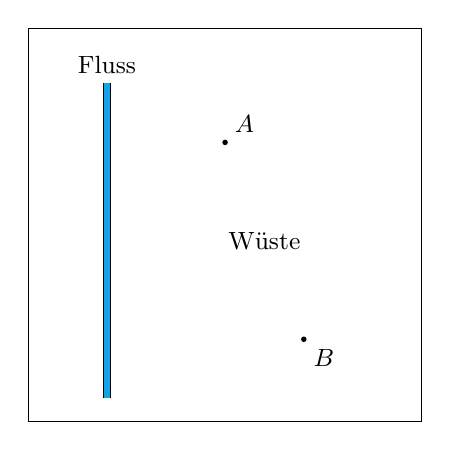
\begin{tikzpicture}
        \clip[draw] (0, 0.2) rectangle (5, 5.2);
        \draw[line width=0.5pt, draw=black, double=Cerulean, double distance=2pt] (1, 0.5) -- (1, 4.5) node[above]{{\small Fluss}};
        \fill (2.5, 3.75) circle(1pt) node[above right]{{\small $A$}};
        \fill (3.5, 1.25) circle(1pt) node[below right]{{\small $B$}};
        \node at (3.0, 2.5) {{\small Wüste}};
      \end{tikzpicture}
    \end{center}
  \fi
  \ifoutline\outline\par
    Denke dir den Fluss (das Flussufer) als Symmetrieachse\ldots
  \fi
  %\ifoutcome\outcome\par
  %\fi
\end{exercise}
